\documentclass[12pt,a4paper]{article}
\usepackage[T1]{fontenc}
\usepackage[utf8]{inputenc}
\usepackage[swedish]{babel}
\usepackage{amsmath}
\usepackage{amsfonts}
\usepackage{amssymb}
\usepackage{lmodern}
\usepackage{hyperref}
\author{Christian Borg Bagge}
\usepackage{parskip}

\usepackage{geometry}
\usepackage{marginnote}

\title{Trädvårdsplan}
\date{2024-11-28}

\begin{document}

\maketitle

\section{Introduktion} 
\label{sec:introduktion}

Petter Krus håller i anförandet och välkomnar deltagarna.
140 deltagare, med ~60\% industri och ~40\% Akademiskt. 
Presentation Akademiskt ~70\% och ~30\% industri.


\subsection{Mål}

\subsubsection{Kultur-ansvar/-historiskt}

\subsubsection{Trivsel}
\subsubsection{Biologiska värden}
\subsubsection{Sociala Värden}
\subsubsection{Dränering/Dagvatten}
\subsubsection{Reducera buller}


\subsection{Ekonomiska}
\subsubsection{Renare luft}
\subsubsection{Skugga}


\subsection{Syfte}

\subsection{Genomförandeidé} 







\section{Indelning}
Pingstliljans samfällighetsförening består av fem olika områden namngivna efter gatunamnen: 



\begin{minipage}{0.5\textwidth}
\vspace{2mm}
\begin{itemize}
	\item Brudslöjan (BR)
	\item Ringblomman (RI)
	\item Pingstliljan (PI)
	\item Lupinen (LU)
	\item Påskliljan (PÅ)
\end{itemize}
\end{minipage}%
\begin{minipage}{0.5\textwidth}
\begin{figure}[h]
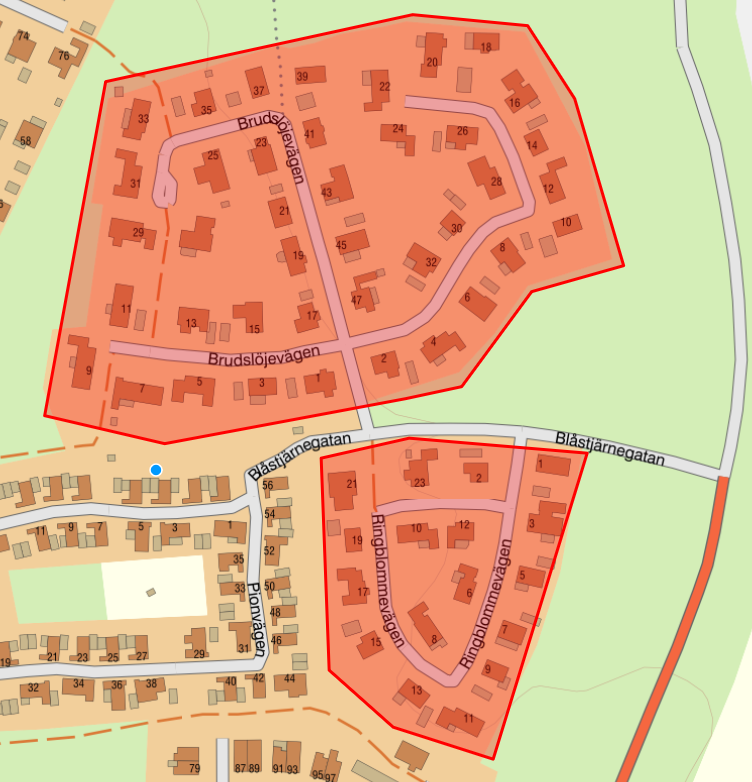
\includegraphics[width=\linewidthcm]{Ring+Brud.png}
\caption{\label{fig:Ring} Ringblomman och Brudslöjans områden}
\end{figure}
Vad kännetecknar området?
Både Ringblomman och Brudslöjan kännetecknas av fristående hus med uppväxta trädgårdar och varierande artbeslag. 

Vad vill vi ha för område?
Sammanfälligheten vill bibehålla trivsamma gemensamma ytor som uppmuntrar till nyttjande och som bidrar till att fungera som gröna lungor. 
Områdets utformning och de större tomterna, där de boende i större grad kan styra sin egen omgivningsmiljö, gör att ambitionsnivån bör vara lägre för de 
gemensamma utrymmena än för de övriga områdena. 

Ett friskt och 

\begin{figure}[h]
\includegraphics[width=\linewidthcm]{Pingst+Lupin+Påsk.png}
\caption{\label{fig:Pingst} Områden Pingstliljan, Lupinen, Påskliljan}
\end{figure}

Vad kännetecknar området?
Pingstliljan, Lupin och Påskliljan kännetecknas av par- eller radhus med med mindre trädgårdar och en stor variation i trädgårdarnas utforming och artbestånd. 
Områdena har ett antal lekparker, aktiva och nedlagda, insprängda bland fastigheterna som skapar större grönområden, en majoritet av dessa grönområden har trädbestånd. 
De aktiva lekparkerna är ett uppskattat inslag för samfällighetens barnfamiljer och nyttjas på regelbundet året runt. 
På grund av yttre påverkan var ett antal träd i mycket dåligt skick och togs ned vintern 23/24. 

Vad vill vi ha för område?
Grönområden har en viktig funktion för att fungera som mötesplats för samfällighetens boende, de bör därför vara en inbjudande miljö. 
I takt med de högre temperaturerna på sommaren och ett förändrat klimat kommer gröna lungor att bli viktigare för att erbjuda svalka och skydd som inte kräver elektrisk effekt.  

De gemenssamma ytorna skall bestå primärt av polinerande lövträd , träd med rotskott skall i det längsta undvikas. 
Omväxlande områden med skugga och sol bestående av träd i olika delar av livscykeln. 
Särskild hänsyn skall tas till faktorer såsom buller, upptag av luftföroreningar och värmebuffert.

%Grönområdena används i stor grad av de familjer i samfälligheten med barn i förskolan eller tidig skolålder. 



\end{minipage}



\section{Avverkning}
\subsection{Påverkan biodepå}
\subsection{Avvägning mellan boende och samfällighet}
Försiktighet, Återhållsamhet och utredning. 

\section{Vårdplan}
Beskrivning av tidsaspekten.
Foto för att bestämma vilka träd som är. 
Foto för att beskriva åtgärder. 

\section{Omfattning}
\subsection{Föryngring}
\subsection{Särskilt skyddsvärda värden}

\end{document}
